\documentclass[11pt]{article}
\usepackage[a4paper,margin=2.5cm]{geometry}
\usepackage[T1]{fontenc}
\usepackage[utf8]{inputenc}
\usepackage{lmodern}
\usepackage{amsmath,amssymb}
\usepackage{graphicx}
\usepackage{booktabs}
\usepackage{multirow}
\usepackage[numbers,sort&compress]{natbib}
\usepackage{xcolor}
\usepackage{tikz}
\usetikzlibrary{arrows.meta,positioning,fit,calc}
\usepackage[hidelinks]{hyperref}
\usepackage{url}
\usepackage{caption}
\captionsetup{font=small,labelfont=bf,justification=raggedright,singlelinecheck=true}

% Generated by paper/make_numbers.py -- do not edit by hand.
\newcommand{\ablDiff}{0.028}
\newcommand{\ablDiffHi}{0.086}
\newcommand{\ablDiffLo}{-0.031}
\newcommand{\ablP}{0.26}
\newcommand{\ablPosOne}{0.214 \pm 0.039}
\newcommand{\ablPosZero}{0.241 \pm 0.021}
\newcommand{\ablRed}{10.8 \pm 19.0}
\newcommand{\ablRedHi}{34}
\newcommand{\ablRedLo}{-13}
\newcommand{\ablRedMax}{29.6}
\newcommand{\ablRedMin}{-16.8}
\newcommand{\ablRotOne}{0.0090 \pm 0.0013}
\newcommand{\ablRotZero}{0.0088 \pm 0.0009}
\newcommand{\ablSeedsNeeded}{25}
\newcommand{\ablWilcoxonP}{0.31}
\newcommand{\ablWins}{3}
\newcommand{\availDown}{36.2}
\newcommand{\availUp}{100}
\newcommand{\benchCfFail}{0.0}
\newcommand{\benchCfMed}{0.232}
\newcommand{\benchCfPninetyfive}{0.607}
\newcommand{\benchDlsEightFail}{0.0}
\newcommand{\benchDlsEightMed}{270.0}
\newcommand{\benchDlsEightPninetyfive}{457.4}
\newcommand{\benchDlsOneFail}{59.5}
\newcommand{\benchDlsOneMed}{136.0}
\newcommand{\benchDlsOnePninetyfive}{260.4}
\newcommand{\benchFasterIkpy}{72}
\newcommand{\benchIkpyFail}{58.0}
\newcommand{\benchIkpyMed}{38.1}
\newcommand{\benchIkpyPninetyfive}{61.9}
\newcommand{\benchNnOneErr}{0.165}
\newcommand{\benchNnOneFail}{0.0}
\newcommand{\benchNnOneMed}{0.531}
\newcommand{\benchNnOnePninetyfive}{1.296}
\newcommand{\benchNnTwoErr}{0.261}
\newcommand{\benchNnTwoFail}{0.0}
\newcommand{\benchNnTwoMed}{4.029}
\newcommand{\benchNnTwoPninetyfive}{7.159}
\newcommand{\benchSlowerCf}{2.3}
\newcommand{\benchTwoHeadsSlower}{8}
\newcommand{\branchesPerTarget}{5.45}
\newcommand{\bugWorst}{784}
\newcommand{\fingerprint}{b9e74b3f67cbfc10}
\newcommand{\fkDiff}{2.5\times 10^{-16}}
\newcommand{\jacMax}{3.2\times 10^{-10}}
\newcommand{\jacRestCond}{16.5}
\newcommand{\jacRestManip}{0.0287}
\newcommand{\mapIn}{0.176}
\newcommand{\mapOut}{14.3}
\newcommand{\mapRatio}{81}
\newcommand{\mapUnreachMax}{1.78}
\newcommand{\mapZ}{0.25}
\newcommand{\mhEightEightKCeil}{100.0}
\newcommand{\mhEightEightKParams}{1,590,320}
\newcommand{\mhEightEightKPos}{0.305 \pm 0.046}
\newcommand{\mhEightEightKRec}{50.6 \pm 9.3}
\newcommand{\mhEightEightKRecMax}{60.8}
\newcommand{\mhEightEightKRecMin}{42.6}
\newcommand{\mhEightEightKRot}{0.25 \pm 0.05}
\newcommand{\mhEightFourKCeil}{74.2}
\newcommand{\mhEightFourKParams}{1,058,840}
\newcommand{\mhEightFourKPos}{0.443 \pm 0.155}
\newcommand{\mhEightFourKRec}{37.8 \pm 13.3}
\newcommand{\mhEightFourKRecMax}{48.8}
\newcommand{\mhEightFourKRecMin}{23.1}
\newcommand{\mhEightFourKRot}{0.39 \pm 0.20}
\newcommand{\mhEightOneCeil}{18.5}
\newcommand{\mhEightOneParams}{660,230}
\newcommand{\mhEightOnePos}{3.18 \pm 4.87}
\newcommand{\mhEightOneRec}{14.2 \pm 7.3}
\newcommand{\mhEightOneRecMax}{18.4}
\newcommand{\mhEightOneRecMin}{5.9}
\newcommand{\mhEightOneRot}{6.22 \pm 10.24}
\newcommand{\mhEightTwoCeil}{37.1}
\newcommand{\mhEightTwoParams}{793,100}
\newcommand{\mhEightTwoPos}{0.413 \pm 0.048}
\newcommand{\mhEightTwoRec}{26.6 \pm 9.3}
\newcommand{\mhEightTwoRecMax}{36.8}
\newcommand{\mhEightTwoRecMin}{18.5}
\newcommand{\mhEightTwoRot}{0.31 \pm 0.02}
\newcommand{\mhFourEightKCeil}{100.0}
\newcommand{\mhFourEightKParams}{1,590,320}
\newcommand{\mhFourEightKPos}{0.381 \pm 0.018}
\newcommand{\mhFourEightKRec}{78.0 \pm 18.7}
\newcommand{\mhFourEightKRecMax}{94.3}
\newcommand{\mhFourEightKRecMin}{57.6}
\newcommand{\mhFourEightKRot}{0.31 \pm 0.01}
\newcommand{\mhFourFourKCeil}{100.0}
\newcommand{\mhFourFourKParams}{1,058,840}
\newcommand{\mhFourFourKPos}{0.308 \pm 0.014}
\newcommand{\mhFourFourKRec}{68.1 \pm 19.2}
\newcommand{\mhFourFourKRecMax}{85.2}
\newcommand{\mhFourFourKRecMin}{47.3}
\newcommand{\mhFourFourKRot}{0.27 \pm 0.06}
\newcommand{\mhFourOneCeil}{37.1}
\newcommand{\mhFourOneParams}{660,230}
\newcommand{\mhFourOnePos}{1.72 \pm 2.31}
\newcommand{\mhFourOneRec}{12.8 \pm 20.9}
\newcommand{\mhFourOneRecMax}{36.9}
\newcommand{\mhFourOneRecMin}{0.0}
\newcommand{\mhFourOneRot}{1.80 \pm 2.54}
\newcommand{\mhFourTwoCeil}{74.2}
\newcommand{\mhFourTwoParams}{793,100}
\newcommand{\mhFourTwoPos}{0.397 \pm 0.042}
\newcommand{\mhFourTwoRec}{32.3 \pm 18.4}
\newcommand{\mhFourTwoRecMax}{48.0}
\newcommand{\mhFourTwoRecMin}{12.1}
\newcommand{\mhFourTwoRot}{0.34 \pm 0.10}
\newcommand{\nSeedsA}{5}
\newcommand{\nSeedsEight}{3}
\newcommand{\nSeedsFour}{3}
\newcommand{\nTargets}{20,201}
\newcommand{\nnMedian}{8.4}
\newcommand{\nnMin}{0.77}
\newcommand{\rtTargets}{2,000}
\newcommand{\shipTestMax}{1.183}
\newcommand{\shipTestMed}{0.164}
\newcommand{\shipTestPninetyfive}{0.426}
\newcommand{\shipTestPos}{0.191}
\newcommand{\shipTestRot}{0.0087}
\newcommand{\splitTest}{2,021}
\newcommand{\splitTrain}{16,160}
\newcommand{\splitVal}{2,020}


\newcommand{\mm}{\,\mathrm{mm}}
\newcommand{\repo}[1]{\texttt{\detokenize{#1}}}
\definecolor{accent}{HTML}{2563EB}

\title{Neural Inverse Kinematics Trained Through a\\
Differentiable Forward Model: A Multi-Seed Study on the UR5e}
\author{Cl\'ement Dumeril\thanks{Personal project, August--September 2026.
Code, data and every result file: \url{https://github.com/clementdumeril/ur5e-neural-kinematics}.
Contact: \texttt{clementdumeril@gmail.com}.}\\[2pt]
{\small University of California, Berkeley (MEng)}}
\date{October 2026}

\begin{document}
\maketitle

\begin{abstract}
A neural network can replace the inverse-kinematics (IK) solver of a robot arm,
but a network trained to regress joint angles is penalised in joint space
rather than where the hand lands. We train a multilayer perceptron for position
IK of a UR5e at a fixed downward tool orientation and backpropagate the
end-effector error through a differentiable Denavit--Hartenberg model in
PyTorch. The deployed network reaches $\shipTestPos\mm$ mean error on
$\splitTest$ held-out targets in $\benchNnOneMed$\,ms. Over $\nSeedsA$ seeds,
adding the forward-kinematics terms to a joint-space loss lowers the test error
by 11\,\% (95\,\% CI $\ablRedLo$ to $+\ablRedHi\,\%$, $p=\ablP$), so an earlier
single-run estimate of 21\,\% does not hold. On data mixing IK branches, a
supervised single-output network collapses, whereas a single output trained on
the forward-kinematics loss alone usually settles on one branch; extra heads
trained with a relaxed winner-take-all loss, without labels, cover more
branches but are not more accurate. The inherited closed-form solver returned
wrong angles for every elbow-down branch (fixed here). The network is
$\benchFasterIkpy\times$ faster than IKPy on the same problem but
$\benchSlowerCf\times$ slower than the closed form, and outside its training
box it returns angles up to $\mapUnreachMax$\,m wrong without warning.
\end{abstract}

%=============================================================================
\section{Introduction}
%=============================================================================
Industrial arms such as the UR5e have closed-form inverse kinematics
\citep{hawkins2013ur}: for a reachable pose the solver returns up to eight
joint configurations in a fraction of a millisecond. Learned IK is therefore
not needed for speed on such arms. It becomes interesting when the solver has to be
differentiable, embedded in a larger learned system, or extended to arms
without an analytic solution \citep{dsouza2001learning,ames2022ikflow}.

The simplest learned IK regresses joint angles from Cartesian targets
\citep{duka2014neural}. The loss is then expressed in joint space: an error of
$10^{-3}$\,rad on the shoulder costs as much as on the last wrist joint,
although the first moves the hand by about a millimetre and the second by
almost nothing. Training the inverse model through a forward model, so that the
error is measured where the hand actually lands, is an old idea
\citep{jordan1992distal}. With automatic differentiation the forward model can
be the robot's exact kinematic chain, which is what physics-informed neural
networks do with differential equations \citep{raissi2019pinn,karniadakis2021piml}.

This paper asks two questions on a simulated UR5e pick-and-place task in
Webots \citep{michel2004webots}: how much does a forward-kinematics (FK) loss
term improve a position-IK network over joint regression, measured on held-out
targets with several seeds; and can a network represent the multi-valued
inverse without being told which solution branch each training sample belongs
to. The contributions are:
\begin{itemize}
  \item a paired, multi-seed ablation of the FK loss term on held-out test
        targets, which shows that its benefit on single-branch data is small
        and not significant at five seeds, contrary to an earlier single-run
        estimate (Section~\ref{sec:results});
  \item a multi-hypothesis IK network trained without branch labels, swept over
        the number of heads on four-branch and eight-branch data, which
        separates accuracy from coverage of the solution set and shows that a
        single head trained on the FK loss alone can already select a branch;
  \item a benchmark against closed-form, damped-least-squares and IKPy solvers,
        a workspace error map that documents silent failure outside the
        training domain, and the correction of a branch-pairing error in the
        inherited closed-form solver.
\end{itemize}

%=============================================================================
\section{Related work}
%=============================================================================
\paragraph{Analytic and numerical IK.}
Kinematic chains are commonly described with Denavit--Hartenberg (DH)
parameters \citep{denavit1955kinematic,siciliano2009robotics}. UR-series arms
admit a closed-form inverse with eight branches, indexed by shoulder, wrist and
elbow configuration \citep{hawkins2013ur}. Iterative solvers linearise the FK
with the Jacobian; damped least squares keeps the step bounded near
singularities \citep{wampler1986dls,nakamura1986singularity,buss2009iksurvey}.
We use both as baselines, together with the IKPy library \citep{manceron_ikpy}.

\paragraph{Learned IK.}
\citet{dsouza2001learning} learn IK locally to sidestep its non-convexity;
\citet{duka2014neural} regress joint angles with a feed-forward network.
\citet{jordan1992distal} train an inverse model through a learned forward
model, the ``distal teacher'', which is the principle used here with an exact,
differentiable FK in place of a learned one. Recent work computes the training
loss in Cartesian space by running FK on predicted joints
\citep{habekost2023cycleik}, or adds an FK-based end-effector cost to a
generative model of robot configurations \citep{lembono2021constrained}.
The term ``physics-informed'' comes from networks whose loss contains
the residual of a governing equation \citep{raissi2019pinn,karniadakis2021piml};
here the ``physics'' is rigid-body kinematics, with no dynamics.

\paragraph{Multi-valued regression.}
When one input has several valid outputs, a least-squares regressor predicts
their mean. Mixture density networks model the conditional density
\citep{bishop1994mdn}; normalising flows and invertible networks sample the
solution set of inverse problems \citep{ardizzone2019inn}, including IK
\citep{ames2022ikflow}; a hypernetwork can also sample joint angles one joint
at a time, conditioned on the target \citep{bensadoun2022nik}. Multiple-choice learning trains several predictors and
updates only the best one per sample
\citep{guzmanrivera2012mcl,lee2016smcl}; relaxing the hard minimum avoids heads
that never train \citep{rupprecht2017uncertain}. Our multi-head network follows
this last line.

%=============================================================================
\section{Problem formulation}
%=============================================================================
\paragraph{Kinematics.}
The UR5e is modelled with the standard DH convention (Table~\ref{tab:dh}). The
forward map $T(q)=\prod_{i=1}^{6} A_i(q_i)\in SE(3)$ gives the tool position
$p(q)$ and orientation $R(q)$; $d_6$ includes a $0.1237$\,m tool offset to the
gripper tip.

\begin{table}[t]
\centering\small
\caption{DH parameters used by all solvers and by the differentiable FK.
Source: \repo{src/kinematics/ur5_pytorch_fk.py}.}
\label{tab:dh}
\begin{tabular}{ccccc}
\toprule
$i$ & $a_i$ (m) & $\alpha_i$ & $d_i$ (m) & $\theta_i$ offset \\
\midrule
1 & 0 & $\pi/2$ & 0.1625 & 0 \\
2 & 0.425 & 0 & 0 & $\pi/2$ \\
3 & 0.3922 & 0 & 0 & 0 \\
4 & 0 & $-\pi/2$ & 0.1333 & $-\pi/2$ \\
5 & 0 & $\pi/2$ & 0.0997 & 0 \\
6 & 0 & 0 & 0.2233 & 0 \\
\bottomrule
\end{tabular}
\end{table}

\paragraph{Task.}
For top-down grasping the tool orientation is fixed to
$R^{\star}=R_{xyz}(\pi,0,-\pi/2)$ (gripper pointing down). The learned map is
therefore position IK, $f_\theta:\mathbb{R}^3\to\mathbb{R}^6$, from a target
$p^{\star}$ in the box $x\in[0,0.4]$, $y\in[-0.9,-0.5]$, $z\in[0.05,0.45]$\,m
above the simulated table. This is not full 6-DoF pose IK: orientation is not
an input.

\paragraph{Multiple solutions.}
For a reachable $(p^\star,R^\star)$ the closed form returns up to eight
configurations, one per choice of shoulder (left/right), wrist (up/down) and
elbow (up/down). A least-squares regressor trained on samples drawn from
several branches converges towards their average, which in general reaches
none of the targets.

%=============================================================================
\section{Method}
%=============================================================================
\begin{figure}[t]
\centering
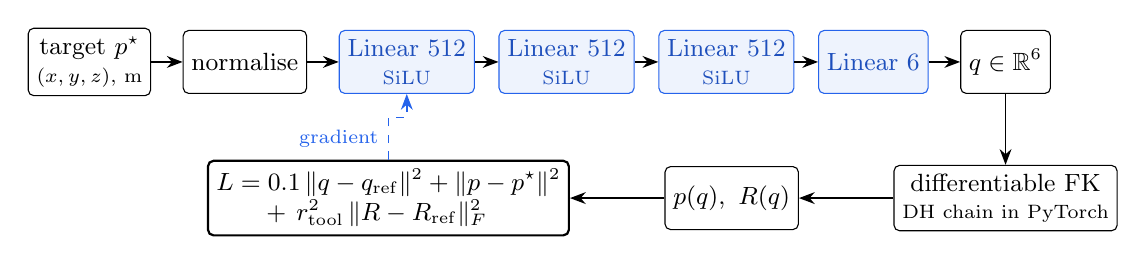
\begin{tikzpicture}[
  box/.style={draw, rounded corners=2pt, minimum height=8mm, inner sep=3pt, font=\small, align=center},
  net/.style={box, draw=accent, fill=accent!8, text=accent!80!black},
  arr/.style={-{Stealth[length=2mm]}, semithick},
  node distance=4mm]
\node[box] (t) {target $p^\star$\\[-1pt]{\scriptsize $(x,y,z)$, m}};
\node[box, right=of t] (n) {normalise};
\node[net, right=of n] (l1) {Linear 512\\[-1pt]{\scriptsize SiLU}};
\node[net, right=3mm of l1] (l2) {Linear 512\\[-1pt]{\scriptsize SiLU}};
\node[net, right=3mm of l2] (l3) {Linear 512\\[-1pt]{\scriptsize SiLU}};
\node[net, right=3mm of l3] (l4) {Linear 6};
\node[box, right=of l4] (q) {$q\in\mathbb{R}^6$};
\node[box, below=9mm of q] (fk) {differentiable FK\\[-1pt]{\scriptsize DH chain in PyTorch}};
\node[box, left=12mm of fk] (pose) {$p(q),\ R(q)$};
\node[box, draw=black, thick, left=12mm of pose, align=left] (L)
  {$L = 0.1\,\|q-q_{\mathrm{ref}}\|^2 + \|p-p^\star\|^2$\\
   $\phantom{L = }+\,r_{\mathrm{tool}}^2\,\|R-R_{\mathrm{ref}}\|_F^2$};
\draw[arr] (t) -- (n); \draw[arr] (n) -- (l1); \draw[arr] (l1) -- (l2);
\draw[arr] (l2) -- (l3); \draw[arr] (l3) -- (l4); \draw[arr] (l4) -- (q);
\draw[arr] (q) -- (fk); \draw[arr] (fk) -- (pose); \draw[arr] (pose) -- (L);
\draw[arr, accent, dashed] (L.north) |- node[pos=0.25, left, font=\scriptsize] {gradient} ($(l1.south)+(0,-3mm)$) -- (l1.south);
\end{tikzpicture}
\caption{Single-output network and training loss. The FK is used only in the
loss; inference is one forward pass. $R_{\mathrm{ref}}=R(q_{\mathrm{ref}})$.}
\label{fig:arch}
\end{figure}

\subsection{Differentiable forward kinematics}
The DH chain of Table~\ref{tab:dh} is implemented as a batched PyTorch module
\citep{paszke2019pytorch}: each $A_i$ is assembled from $\cos q_i$, $\sin q_i$
and constants, and the six transforms are chained with batched matrix
products. The module agrees with the inherited NumPy FK to
$\fkDiff$\,m on 1,000 random configurations (Section~\ref{sec:verif}).

\subsection{Network and loss}
$f_\theta$ is an MLP with three hidden layers of 512 units and SiLU activations
\citep{elfwing2018silu} (530,438 parameters, Figure~\ref{fig:arch}). SiLU was
chosen because the loss gradient passes through the sines and cosines of the
FK and a smooth activation keeps it continuous; it was not compared against
ReLU. Input and output normalisation statistics are stored in the checkpoint.
The loss is
\begin{equation}
L(\theta) = w_d\,\|q-q_{\mathrm{ref}}\|^2
 + w_p\left(\|p(q)-p^\star\|^2 + r_{\mathrm{tool}}^2\,\|R(q)-R(q_{\mathrm{ref}})\|_F^2\right),
\qquad q=f_\theta(p^\star),
\label{eq:loss}
\end{equation}
with $w_d=0.1$, $w_p=1$ and $r_{\mathrm{tool}}=0.05$\,m, all terms averaged
over the batch. Three choices matter:
(i) the data term anchors the network to one IK branch;
(ii) the orientation reference is $R(q_{\mathrm{ref}})$ rather than a matrix
rebuilt from Euler angles, so both sides pass through the same kinematics;
without an orientation term a $\pi$ rotation of $q_6$ flips the gripper at zero
position cost;
(iii) the Frobenius norm avoids the $\arccos$ of the geodesic distance, whose
gradient diverges at zero error. Weighting by $r_{\mathrm{tool}}^2$ converts a
rotation into the displacement it causes at a $5$\,cm lever arm, so both terms
are in m$^2$.

\subsection{Multi-hypothesis network}
For branch-mixed data a shared trunk (three layers of 512, SiLU) feeds $K$
heads ($512\to256\to6$), giving proposals $q^{(1)},\dots,q^{(K)}$. With
$\ell_k$ the FK pose error of head $k$ (position plus $r_{\mathrm{tool}}^2$
times the Frobenius rotation error, no data term), the loss is the relaxed
minimum
\begin{equation}
L_{\mathrm{MH}} = (1-\varepsilon)\,\ell_{k^\star} + \frac{\varepsilon}{K-1}\sum_{k\neq k^\star}\ell_k,
\qquad k^\star=\arg\min_k \ell_k,\quad \varepsilon=0.05,
\end{equation}
so losing heads still receive gradient \citep{rupprecht2017uncertain}. No
branch label enters training. At inference the FK scores the $K$ proposals with
the same pose error and the best one is returned. Branch recall is the share
of valid closed-form solutions that at least one head lies within 0.25\,rad of,
under a periodic angular distance in joint space. It measures how many branches
the proposals point to, not that every proposal reaches the target: only the
selected head is held to the pose error, and 0.25\,rad at the shoulder moves
the tool by roughly 0.2\,m. With $K$ heads and $n_i$ valid branches for target
$i$, recall cannot exceed $\sum_i \min(K,n_i)/\sum_i n_i$.

\subsection{Data}
Targets are drawn uniformly in the box. For each target the closed form is
evaluated on every branch and a solution is kept only if its FK reaches the
target; filtering on NaN is not enough (Section~\ref{sec:verif}). The cached
data set has $\nTargets$ reachable targets (fingerprint \texttt{\fingerprint}).
The deployed checkpoint was trained by \repo{train_true_pinn.py} on a
separately generated set of the same distribution, using the
left--up--up branch only.

\subsection{Protocol}
Adam \citep{kingma2015adam}, learning rate $10^{-3}$ divided in steps to
$2\times10^{-5}$ at epochs 30, 60 and 80, batch 256, 100 epochs. All
experiments in Section~\ref{sec:results} use a fixed random split into
$\splitTrain$ training, $\splitVal$ validation and $\splitTest$ test targets;
the epoch is selected on validation position error and all reported errors
are test errors. Errors are the mean Euclidean distance between the pose
reached by FK and the target, and the mean geodesic angle to $R(q_{\mathrm{ref}})$.
Seeds change only the initialisation and the batch order; the data and the
split are the same for every run, so the reported spread does not include
the variance due to data sampling.

\subsection{Baselines and integration}
The closed form is the inherited solver with the correction of
Section~\ref{sec:verif}. Damped least squares uses the geometric Jacobian with
adaptive damping driven by the smallest singular value and an SO(3) logarithm
for the rotation error, from one start or with eight random restarts. For
IKPy \citep{manceron_ikpy} we build the chain from the DH table of
Table~\ref{tab:dh} (its FK matches ours to $10^{-15}$), impose the full tool
orientation and start from the same rest configuration as damped least
squares, so all solvers face the same problem on the same targets. A solution
further than 1\,mm or $0.1^\circ$ from the requested pose counts as a failure.
Timing uses 200 targets, after 200 warm-up calls on a different set. In Webots the camera reads the cube position through a homography
fitted with RANSAC \citep{fischler1981ransac,hartley2004mvg} on a calibration
grid, the network solves each grasp and transport target, and quintic
trajectories with a closed-loop joint-position hold drive the arm.

%=============================================================================
\section{Verification}
\label{sec:verif}
%=============================================================================
\paragraph{Kinematic consistency.}
The PyTorch FK matches the NumPy FK to $\fkDiff$\,m in position over 1,000
random configurations. The analytic geometric Jacobian, built column by column
from $J_{v,i}=z_{i-1}\times(p_e-p_{i-1})$, $J_{\omega,i}=z_{i-1}$, matches a
central finite-difference derivative of the FK to $\jacMax$ (maximum absolute
entry difference, 200 random configurations). At the rest pose its
manipulability is $\jacRestManip$ and its condition number $\jacRestCond$; at
the fully extended configuration $q=0$ the manipulability is zero, as expected.

\paragraph{A branch-pairing error in the closed-form solver.}
Round-tripping $\mathrm{FK}(\mathrm{IK}(p))$ on $\rtTargets$ targets showed that
the inherited closed form returned finite angles for every elbow-down branch,
all of them wrong, up to $\bugWorst\mm$ from the target. The solver chose
$\theta_2$ from the shoulder configuration only, while $\theta_3$ depended on
the elbow; pairing $\theta_2$ with the elbow choice brings all eight branches
to round-trip errors below $10^{-9}$\,m. Before the fix, the FK filter of the
data generator removed these solutions, so the published four-branch
experiment (Part~B below) only contained elbow-up branches. The fix does not
change any single-branch result: the deployed model, the ablation and the
benchmark use the left--up--up branch, which the error did not affect. A
regression test now round-trips all eight branches.

\paragraph{Data and evaluation.}
Training, validation and test indices are disjoint; the nearest training
target to a test target is $\nnMin\mm$ away at minimum and $\nnMedian\mm$ at
the median. Timings discard 200 warm-up calls made on separate targets, run on one thread and include the
NumPy-to-tensor conversion a caller pays. A smoke test covering imports, data
paths, a known target, the camera calibration and the eight-branch round trip
runs in continuous integration.

%=============================================================================
\section{Results}
\label{sec:results}
%=============================================================================
\subsection{Deployed model}
On the $\splitTest$ test targets, which it never saw, the deployed checkpoint
reaches $\shipTestPos\mm$ mean position error (median $\shipTestMed\mm$,
95th percentile $\shipTestPninetyfive\mm$, maximum $\shipTestMax\mm$) and
$\shipTestRot^\circ$ mean orientation error. Its validation error at the
selected epoch, on the set used for selection, was $0.185\mm$.

\subsection{Effect of the forward-kinematics terms}
Table~\ref{tab:abl} and Figure~\ref{fig:abl} compare $w_p=0$ (data term only)
with $w_p=1$ on single-branch data. The mean test position error goes from
$\ablPosZero\mm$ to $\ablPosOne\mm$. Paired by seed, the FK terms help in
$\ablWins$ of $\nSeedsA$ seeds; the mean difference is $\ablDiff\mm$, with a
95\,\% confidence interval of $[\ablDiffLo, \ablDiffHi]\mm$ (paired $t$-test,
$p=\ablP$; Wilcoxon signed-rank $p=\ablWilcoxonP$, whose smallest attainable
value with five pairs is 0.0625), and the relative reduction ranges from
$\ablRedMin$ to $\ablRedMax\,\%$ across seeds. Orientation error stays near
one hundredth of a degree in both cases. At this sample size the FK terms do
not give a reliable gain on single-branch data; detecting the observed mean
difference with 80\,\% power at the 5\,\% level would take about
$\ablSeedsNeeded$ paired seeds. An earlier single run reported a
21\,\% reduction; it used one seed and selected and reported the epoch on the
same validation set. The single-branch target is a smooth function of the
position, which the data term alone already fits to a quarter of a millimetre;
the run-to-run spread of the network is of the same order as the effect.

\begin{table}[t]
\centering\small
\caption{FK-term ablation on single-branch data, test split, mean $\pm$ standard
deviation over $\nSeedsA$ seeds (\repo{results/seed_study/A_*.json}).}
\label{tab:abl}
\begin{tabular}{lcc}
\toprule
Loss & Position (mm) & Orientation (deg) \\
\midrule
data term only ($w_p=0$) & $\ablPosZero$ & $\ablRotZero$ \\
data + FK terms ($w_p=1$) & $\ablPosOne$ & $\ablRotOne$ \\
\midrule
paired reduction in position & \multicolumn{2}{c}{$\ablRed\,\%$} \\
\bottomrule
\end{tabular}
\end{table}

\begin{figure}[t]
\centering
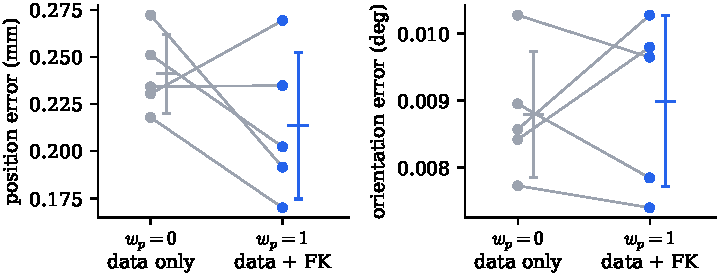
\includegraphics[width=0.72\linewidth]{figures/ablation.pdf}
\caption{Test error per seed with and without the FK terms; lines join runs
with the same seed, bars show mean $\pm$ one standard deviation.}
\label{fig:abl}
\end{figure}

\subsection{Multi-valued IK without branch labels}
Table~\ref{tab:mh} and Figure~\ref{fig:mh} report the multi-head network on
branch-mixed data. Part~B uses the four elbow-up branches (the data set of the
original experiment); Part~D uses all eight branches after the solver
correction, with on average $\branchesPerTarget$ valid branches per target.

With three seeds per configuration these results are descriptive. With $K=1$
the loss contains no data term, so nothing pulls the single output towards the
average of the branches: in two of three seeds on each data set it settles on
one branch and reaches 0.33--0.44\,mm, and in the third it stalls between
branches at 4.4 and 8.8\,mm. This suggests that the collapse to the average
reported in the original ablation (911\,mm) comes from the supervised data
term on mixed labels rather than from the single-output architecture. From
$K=2$ every run is sub-millimetre (0.26--0.62\,mm) and the error does not
improve systematically with more heads. Recall grows with $K$, from
$\mhFourOneRec$ to $\mhFourEightKRec\,\%$ on four branches and from
$\mhEightOneRec$ to $\mhEightEightKRec\,\%$ on eight, against ceilings of
$\mhFourOneCeil$ to $\mhFourEightKCeil\,\%$ and $\mhEightOneCeil$ to
$\mhEightEightKCeil\,\%$: best-of-$K$ needs one correct proposal, whereas
covering the solution set needs one head per branch. Which branches are
covered varies from seed to seed. On the four-branch set, a head that
lands on an elbow-down solution counts as a miss, because those branches are
absent from that data set. This is the likely reason one $K=1$ run reaches
0.44\,mm with zero recall; the weights of these runs were not stored, so it
was not checked directly.

\begin{table}[t]
\centering\small
\caption{Multi-head IK on branch-mixed data, test split, mean $\pm$ standard
deviation over three seeds (\repo{results/seed_study/B_*.json, D_*.json}).
Recall: share of valid branches that at least one head lies within 0.25\,rad of;
ceiling: highest recall attainable with $K$ heads on the test targets.}
\label{tab:mh}
\begin{tabular}{llcccc}
\toprule
Data & $K$ & Position (mm) & Orientation (deg) & Recall (\%) & Ceiling (\%) \\
\midrule
\multirow{4}{*}{4 branches (B)}
 & 1 & $\mhFourOnePos$ & $\mhFourOneRot$ & $\mhFourOneRec$ & $\mhFourOneCeil$ \\
 & 2 & $\mhFourTwoPos$ & $\mhFourTwoRot$ & $\mhFourTwoRec$ & $\mhFourTwoCeil$ \\
 & 4 & $\mhFourFourKPos$ & $\mhFourFourKRot$ & $\mhFourFourKRec$ & $\mhFourFourKCeil$ \\
 & 8 & $\mhFourEightKPos$ & $\mhFourEightKRot$ & $\mhFourEightKRec$ & $\mhFourEightKCeil$ \\
\midrule
\multirow{4}{*}{8 branches (D)}
 & 1 & $\mhEightOnePos$ & $\mhEightOneRot$ & $\mhEightOneRec$ & $\mhEightOneCeil$ \\
 & 2 & $\mhEightTwoPos$ & $\mhEightTwoRot$ & $\mhEightTwoRec$ & $\mhEightTwoCeil$ \\
 & 4 & $\mhEightFourKPos$ & $\mhEightFourKRot$ & $\mhEightFourKRec$ & $\mhEightFourKCeil$ \\
 & 8 & $\mhEightEightKPos$ & $\mhEightEightKRot$ & $\mhEightEightKRec$ & $\mhEightEightKCeil$ \\
\bottomrule
\end{tabular}
\end{table}

\begin{figure}[t]
\centering
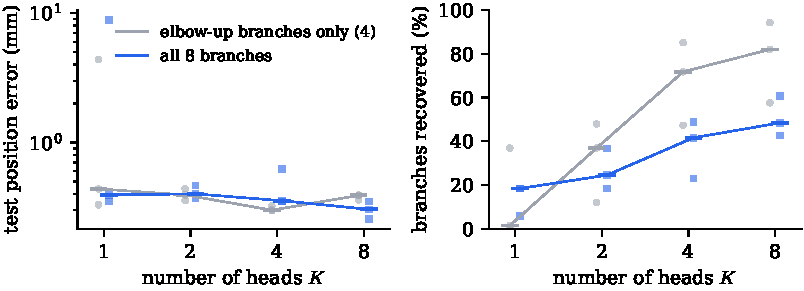
\includegraphics[width=0.9\linewidth]{figures/multihead.pdf}
\caption{Multi-head sweep. Points are seeds, short bars medians. Left: test
position error (log scale). Right: branch recall.}
\label{fig:mh}
\end{figure}

\subsection{Solver benchmark}
Figure~\ref{fig:bench} and Table~\ref{tab:bench} compare solve times on 200
targets. The closed form is the fastest at $\benchCfMed$\,ms. The single-output
network takes $\benchNnOneMed$\,ms, $\benchSlowerCf\times$ slower. The two
generic iterative solvers behave alike from the rest configuration: damped
least squares fails on $\benchDlsOneFail\,\%$ of targets and IKPy, solving the
same pose problem, on $\benchIkpyFail\,\%$, both stalling in local minima. IKPy
takes $\benchIkpyMed$\,ms, $\benchFasterIkpy\times$ the network's time; eight
restarts remove the failures of damped least squares at roughly twice its cost. The two-head network is $\benchTwoHeadsSlower\times$
slower than the single-output one, mostly because inference must run the FK on
every proposal.

\begin{figure}[t]
\centering
\begin{minipage}[c]{0.48\linewidth}
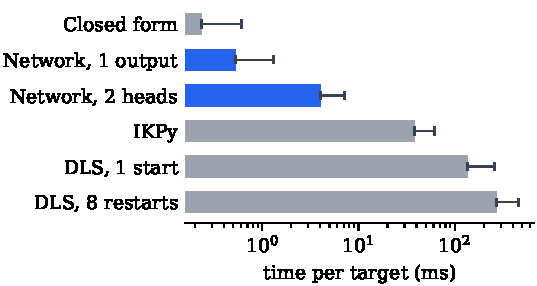
\includegraphics[width=\linewidth]{figures/benchmark.pdf}
\end{minipage}\hfill
\begin{minipage}[c]{0.49\linewidth}
\small
\begin{tabular}{lrrr}
\toprule
Solver & Median & p95 & Fail. \\
 & (ms) & (ms) & (\%) \\
\midrule
Closed form & $\benchCfMed$ & $\benchCfPninetyfive$ & $\benchCfFail$ \\
Network, 1 out. & $\benchNnOneMed$ & $\benchNnOnePninetyfive$ & $\benchNnOneFail$ \\
Network, 2 heads & $\benchNnTwoMed$ & $\benchNnTwoPninetyfive$ & $\benchNnTwoFail$ \\
IKPy & $\benchIkpyMed$ & $\benchIkpyPninetyfive$ & $\benchIkpyFail$ \\
DLS, 1 start & $\benchDlsOneMed$ & $\benchDlsOnePninetyfive$ & $\benchDlsOneFail$ \\
DLS, 8 restarts & $\benchDlsEightMed$ & $\benchDlsEightPninetyfive$ & $\benchDlsEightFail$ \\
\bottomrule
\end{tabular}
\end{minipage}
\caption{Solve time per target (bars: median; whiskers: 95th percentile) on the
same 200 pose targets, one thread, after
200 warm-up calls on other targets (\repo{results/benchmark/benchmark.json}).
Failure: more than 1\,mm or $0.1^\circ$ from the requested pose. Median network
errors: $\benchNnOneErr\mm$ (single output) and $\benchNnTwoErr\mm$ (two heads).}
\label{fig:bench}\label{tab:bench}
\end{figure}

\subsection{Behaviour outside the training domain}
Figure~\ref{fig:map} maps the deployed network's error on a horizontal slice at
$z=\mapZ$\,m. The median error is $\mapIn\mm$ inside the training box and
$\mapOut\mm$ at reachable points outside it, $\mapRatio\times$ larger. Past the
reach limit, where the closed form raises an exception, the network still
returns six angles, up to $\mapUnreachMax$\,m wrong. Along a line at
$y=-0.70$\,m, $z=0.25$\,m the error of the returned pose is 0.2\,mm at
$x=0.40$, 2.0\,mm at $0.50$, then 68, 389 and 1460\,mm at $0.55$, $0.60$ and
$0.70$\,m, where no solution exists (\repo{results/verification/continuity_log.txt}).

\begin{figure}[t]
\centering
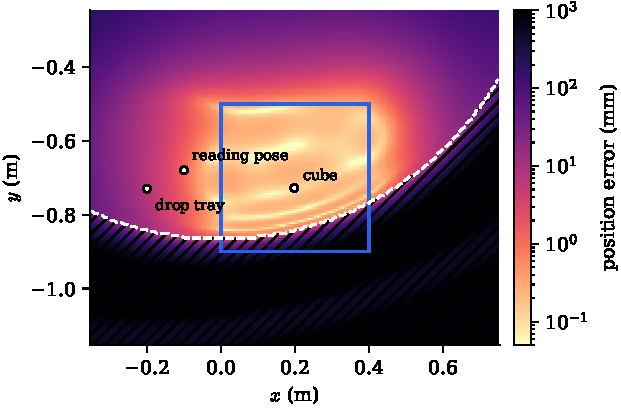
\includegraphics[width=0.62\linewidth]{figures/workspace_error.pdf}
\caption{Position error of the deployed network at $z=\mapZ$\,m (log colour
scale). Blue: training box. Dashed: reach limit of the closed form; hatched:
no solution exists.}
\label{fig:map}
\end{figure}

\paragraph{Continuity.}
Along a 400-sample circle inside the workspace, the network and the closed form
give identical joint-space steps (median 0.0084\,rad) and no branch change. With
the tool pointing down the preferred branch is valid everywhere on the path, so
the network has no continuity advantage here.

\subsection{Closed-loop simulation}
In Webots (Figure~\ref{fig:webots}) the arm locates the cube with its camera
and the network solves every move to the cube and to the tray; only the camera
reading pose, outside the training box, uses the closed form. After the
scenario, a campaign drives the arm to each scenario target with the closed
form, again with the closed form (repeatability), and with the network, and
compares the poses reached in the physics engine. With the deployed checkpoint
(Webots R2025a, \repo{results/webots/closed_loop_console.txt}) the network is
$0.45\mm$ off above the cube and $0.33\mm$ at the grasp point, against a
repeatability of at most 0.04\,mm, and 10.9 and 7.3\,mm above the tray. The
tray, at $x=-0.20$\,m, lies outside the training box, yet the network drives
the arm there; the drop tolerates the error. Each value is a single target. In
the same run the camera located the cube, the grasp lifted it by 369\,mm and
the cube reached the tray. A homography fitted on a calibration grid maps
pixels to the table with a 1.1\,mm median residual, and a colour-threshold
detector located the cube within 8\,mm, against 49\,mm for a VGG16 regressor,
which was dropped.

\begin{figure}[t]
\centering
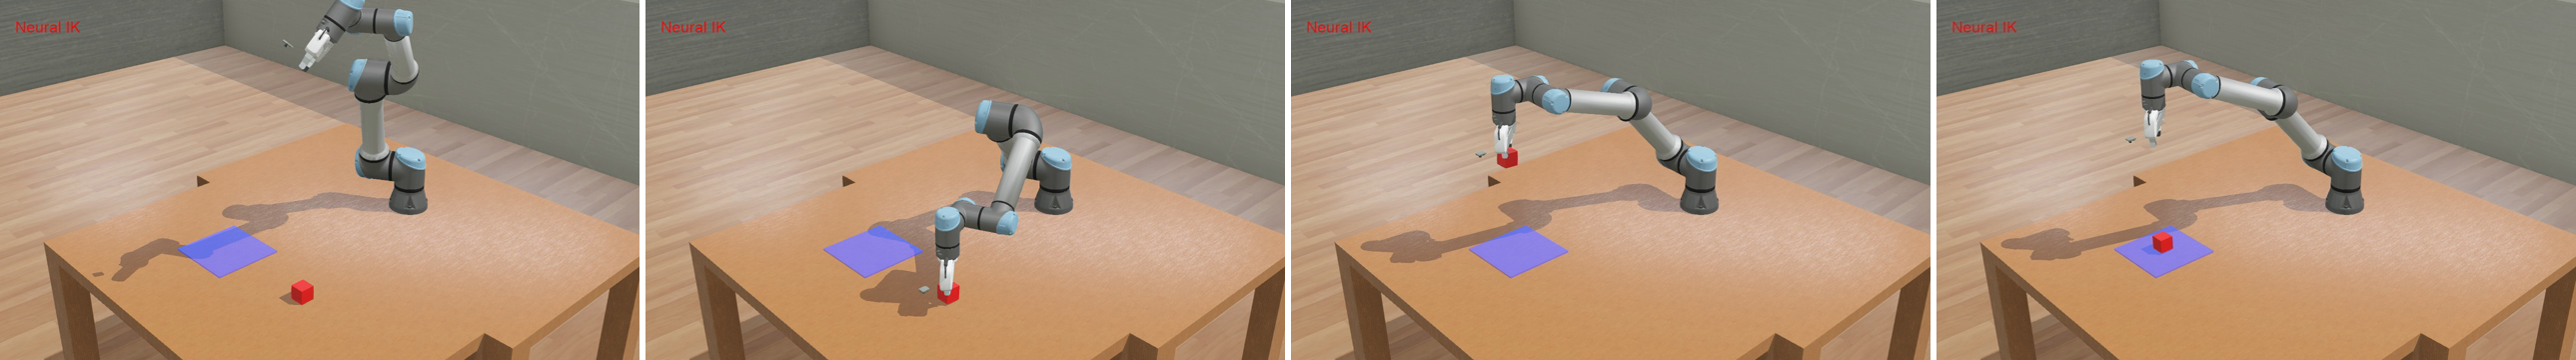
\includegraphics[width=\linewidth]{figures/webots_sequence.png}
\caption{One closed-loop run in Webots with the deployed network: reading pose
(the camera locates the cube), grasp, transport, cube on the tray. Frames of the
movie recorded by \repo{webots/controllers/capture_recorder}.}
\label{fig:webots}
\end{figure}

%=============================================================================
\section{Discussion and limitations}
%=============================================================================
\paragraph{What the results support.}
A position-IK network trained through a differentiable FK reaches about
0.2\,mm on held-out targets inside its training box. A loss computed on the reached
pose, rather than on joint labels, lets the network cope with a multi-valued
inverse: one head picks a branch on its own most of the time, and several
heads trained without labels cover a growing share of the solution set.

\paragraph{What they do not support.}
\begin{itemize}
\item \emph{A gain from the FK terms on single-branch data.} With five seeds the
  paired difference is not significant; more seeds or a larger effect would be
  needed to claim one.
\item \emph{Pose IK.} The network maps positions to joints at one fixed tool
  orientation. Full 6-DoF IK would take the orientation as input and needs new
  data.
\item \emph{Speed.} The network is $\benchSlowerCf\times$ slower than the closed
  form. Its speed advantage holds only against generic iterative solvers.
\item \emph{Safety.} Outside the training box the error grows by orders of
  magnitude and the network gives no signal. A reachability and domain check
  must sit in front of it; the present pick-and-place loop does not have one
  and sends the network to the tray, outside its training box.
\item \emph{Multi-head trade-off.} On this task, fixing the branch in the data
  generator is simpler and more accurate than learning it; the multi-head
  model becomes useful when the branch cannot be chosen in advance, for
  instance with several tool orientations or obstacle constraints. Which
  branches the heads cover varies between seeds.
\item \emph{Physical validity of branches.} Branches are counted when the FK
  reaches the target; joint limits and collisions with the table are not
  checked, so some elbow-down solutions may not be executable.
\item \emph{Scope of measurement.} Results come from kinematic evaluation and
  one simulator; the closed-loop figures are single targets from one run, and
  the workspace map is a single horizontal slice.
\item \emph{Naming.} The loss contains no dynamics or differential operator;
  ``physics-informed'' here means kinematics-informed.
\end{itemize}

%=============================================================================
\section{Conclusion and future work}
%=============================================================================
On a single IK branch, backpropagating the end-effector error through an exact
differentiable FK did not give a reliable gain over joint regression once
seeds and a held-out test set were taken into account. On mixed data, only a
pose loss trains without labels; a single head avoided the collapse to the
average in four of six runs, and a relaxed winner-take-all multi-head network
covered more of the solution set, at no gain in accuracy. The network remains
slower than the closed form and unsafe outside its domain. Natural next steps are an orientation input for pose IK, an
explicit reachability or confidence output, joint-limit and collision checks
on the recovered branches, and a closed-loop evaluation over many targets
rather than the four of the scenario.

%=============================================================================
\section*{Reproducibility statement}
%=============================================================================
Code, checkpoints, cached-data fingerprints and all result files are in the
repository. Hardware: Intel Core i7-6700HQ (4 cores), 32\,GB RAM, no GPU.
Software: Python 3.11.9, PyTorch 2.8.0 (CPU), NumPy 2.2.6, SciPy 1.15.2,
Matplotlib 3.10.6, IKPy 4.0.0, Webots R2025a, MiKTeX pdf\TeX{} 4.23.
\begin{center}\small
\begin{tabular}{ll}
\toprule
Command & Time \\
\midrule
\texttt{python experiments/verify\_paper.py} & 1 min \\
\texttt{python experiments/seed\_study.py} (Parts A--C) & 3 h \\
\texttt{SEED\_PART=D python experiments/seed\_study.py} & 2.5 h \\
\texttt{python experiments/benchmark\_solveurs.py} & 6 min \\
\texttt{python experiments/mesure\_continuite.py} & 1 min \\
\texttt{python paper/make\_figures.py \&\& python paper/make\_numbers.py} & 4 min \\
\texttt{cd paper \&\& latexmk -pdf main.tex} & 1 min \\
\bottomrule
\end{tabular}
\end{center}
Every number in this paper is either copied by hand from the file cited next
to it or
generated into \repo{paper/numbers.tex} by \repo{paper/make_numbers.py}.

\bibliographystyle{plainnat}
\bibliography{references}

\end{document}
